\documentclass{report}
\usepackage{hyperref}
\usepackage[utf8]{inputenc}
\usepackage{graphics}
\graphicspath{ {./images/} }
\usepackage{multicol}
\usepackage{array}

\usepackage[a4paper, total={7in, 10in}]{geometry}

\title{IOT - CIA1}
\author{Akshay S G}
\date{\today}

\begin{document}

    \begin{titlepage}
    \centering
        \vspace*{2cm}
        \Huge
        \textbf{Smart Doorbell Monitoring System}
        
        \vspace*{0.6cm}
        \Large
        \textit{}
        
        \Large
        \vspace*{1.5cm}
        Akshay S G\\
        \vspace{0.2cm}
        21011101017\\
        \vspace{0.2cm}
        AI-DS A\\
        
        \vfill              
        
        \vfill
        
        %\includegraphics[scale=0.5]{logo}
        
        
\includegraphics{images/snu.png}\\
        B.Tech Artificial Intelligence and Data Science\\
        Shiv Nadar University, Chennai\\
        20 January 2023
        \vspace*{1cm}
    
\end{titlepage}

    
    \begin{center}
        \section*{Smart Doorbell Monitoring System}
    \end{center}
\setlength{\columnsep}{1.0cm}
    \large
    \section{Summary}
    A smart doorbell system is a device that is installed on the exterior of a home or building and allows the user to monitor and interact with visitors remotely. The system typically includes a camera, speaker, and microphone, as well as a connection to the internet. When a visitor rings the doorbell, the camera gets triggered and captures their face and it checks for their face with the database which already has registered faces, when an unauthorized person is detected, it alerts the user through a text message. This allows the user to monitor the front of their home or building even when they are not at home. Overall, a smart doorbell system provides a convenient way for homeowners and building managers to monitor and interact with visitors remotely and provides added security benefits.
\section{Design And Work Process}
\begin{multicols}{1}    
    \begin{enumerate}    
        \item Design concept: \\
        The paper presents an intelligent doorbell system that utilizes human face identification as the primary method of operation. The system employs face detection and subsequently compares the detected face to entries in a database 
        to identify the individual. The system is demonstrated with an example in Figure 1.
        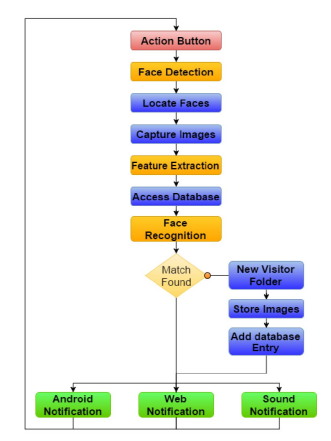
\includegraphics{images/system_procedures.png}\\
        \makebox[8cm][r]{Fig 2 : Flowchart of system procedures}\\
        \item Face Detection: \\
        This section of the paper discusses the process of resolving images to determine whether human faces appear and pinpoint their location for cropping, using Haar-like features and looping through the image to identify and locate faces for cropping. Filters such as face alignment and scaling are applied to improve the algorithm's effectiveness.
        \item Feature Extraction: \\
        This section discusses the process of extracting human-face patches from images after detection. Feature extractions are implemented to reduce dimension, improve conspicuous extraction, and decrease noise. The face image is transformed into a fixed-dimension vector and stored in an XML or PCD file. The faces are described as polygons or objects.
        \item Feature Recognition: \\
        This section describes the process of applying a matching algorithm between the stored data and the input image.Two main applications are established: identification and verification. Identification allows the system to recognize the person through a given face image using the Eigenface algorithm. Verification, on the other hand, differentiates if a given face image matches or not with a guess face to improve the verification. The steps of face recognition are illustrated in Figure 2.
        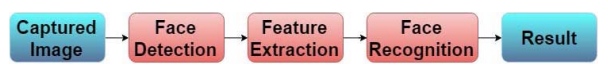
\includegraphics{images/face_recognition.png}\\
        \makebox[2cm][r]{\rule{0pt}{3cm}{Figure 3. Face recognition procedures}}
    \end{enumerate}
\end{multicols}

\vspace*{0.6cm}
\small
\textit{}

\begin{multicols}{1} 
    \section{IOT Architecture}
    This paper aims to discuss the development of an enhanced smart doorbell system based on face recognition technology and IoT (Internet of Things) device. The system utilizes biometrics to map facial features from a photograph or video and compares the information with a database of known faces to find a match. The main goal of this work is to form an intelligent doorbell system based on human face identification, in order to enhance security and improve home automation.\\ 

    The system utilizes the OpenCV library and replaces costly image processing boards by using a \textbf{Raspberry pi board} with ARMv7 Cortex-A7 as the core.e face recognition process is initiated by pressing the doorbell button, where an \textbf{integrated camera} integrated camera captures several pictures of the visitor. The recently scanned face is then verified in the present database. In case of an unknown face, the {principal component analysis (PCA), the \textbf{GSM Module}, an IoT device that is connected to the internet and can send notifications to the owner's mobile phone is programmed and implemented on the platform.\\ 

    
        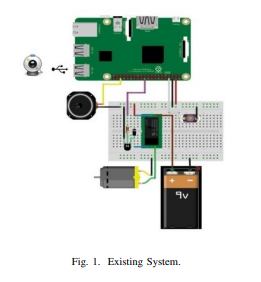
\includegraphics{images/doorbell.png}\\
        
    Let us talk in detail about the three IOT devices used and their architecture: \\
    
        \textbf{Raspberry pi board} : \\ \\
        The architecture of the Raspberry Pi is based on a Broadcom system-on-a-chip (SoC) which includes an ARM-compatible central processing unit (CPU) and an on-chip graphics processing unit (GPU).
        The Raspberry Pi uses a 40-pin GPIO (General Purpose Input/Output) header to connect to various peripheral devices such as sensors, actuators, and other electronic components. The 40 pins include \\ \\   
        \begin{tabular}{ | m{6em} | m{5cm} | } 
            \hline
            \textbf Components  & Architecture\\ 
            \hline
            Central Processing Unit (CPU) & This is the main processor that runs the operating system and executes instructions. \\ 
            \hline
            Memory & This is the storage area where the operating system and programs are stored.\\ 
            \hline
           Input/Output (I/O) interfaces & These are the interfaces that allow the Raspberry Pi to communicate with other devices and peripherals.\\
            \hline
        \end{tabular}

\scalebox{0.3}{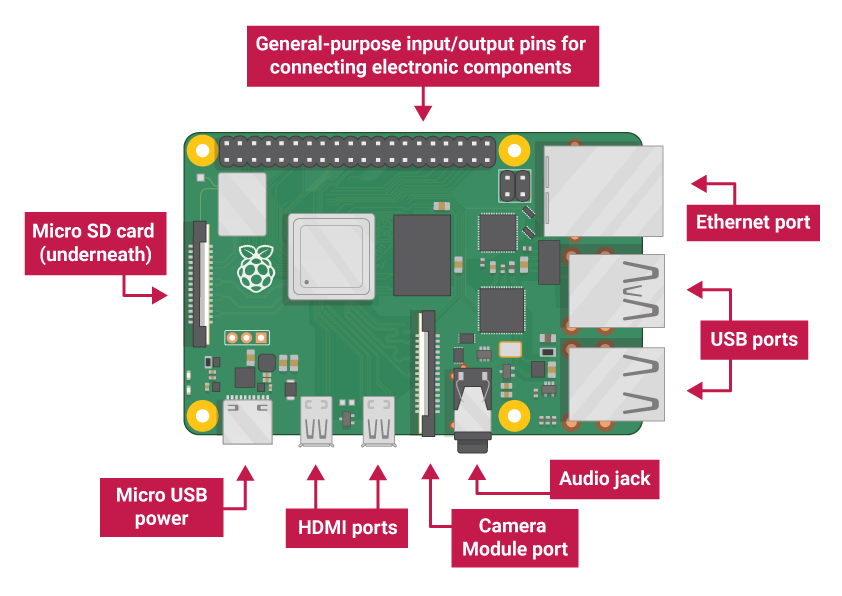
\includegraphics{images/rasberry_pi.png}}
\makebox[7cm][r]{\rule{0pt}{0cm}{Figure 4. Raspberry Pi Architecture}}

        The Raspberry Pi uses a variety of communication protocols to interact with other devices and peripherals, including: \\

        \begin{tabular}{ | m{6em} | m{5cm} | } 
                \hline
                \textbf Protocol Layers & Protocol in the stacks\\ 
                \hline
                Ethernet & The Raspberry Pi can be connected to a wired network using an Ethernet cable and an Ethernet port. \\ 
                \hline
                WiFi & The Raspberry Pi can connect to wireless networks using built-in WiFi or a USB wireless adapter.\\ 
                \hline
                Bluetooth & The Raspberry Pi can connect to Bluetooth devices using built-in Bluetooth or a USB Bluetooth adapter.\\
                \hline
        \end{tabular}
        \begin{tabular}{ | m{6em} | m{5cm} | } 
                \hline
                \textbf Protocol Layers & Protocol in the stacks\\ 
                \hline
                USB & The Raspberry Pi can connect to a variety of devices using USB ports, including keyboards, mice, and storage devices.\\
                \hline                
                GPIO (General Purpose Input/Output) & he Raspberry Pi has a 40-pin header that can be used to connect to a variety of sensors and other devices using a variety of protocols such as I2C, SPI, UART.\\
                \hline
                HDMI & The Raspberry Pi can connect to a monitor or TV using HDMI to display video and audio.\\
                \hline
                RCA & The Raspberry Pi can connect to a monitor or TV using RCA for video.\\
                \hline
        \end{tabular}
        

        
\vspace*{0.3cm}
\textit{}

        The Raspberry Pi also includes various built-in interfaces such as Ethernet, HDMI, USB, and a 3.5mm audio jack, as well as a microSD card slot for storage. The device runs on a Linux-based operating system, and can be programmed using various programming languages such as Python, C, and Java. \\ \\ 

        \textbf{Intergrated Camera} : \\
         Integrated cameras are typically built using a combination of hardware and software components. The hardware components typically include an image sensor, optics, and a lens. The software components include the camera driver and the application programming interfaces (APIs) that allow the camera to communicate with other devices and software.\\

         The architecture of an integrated camera can vary depending on the specific camera and the platform it is used on. However, a typical architecture includes the following components: \\ 
  
        \begin{tabular}{ | m{6em} | m{5cm} | } 
            \hline
            \textbf Components  & Architecture\\ 
            \hline
            Image sensor & This is the hardware component that captures the light and converts it into an electrical signal. \\ 
            \hline
            Lens & This is the optical component that focuses the light onto the image sensor.\\ 
            \hline
            Image processor & This is the hardware component that processes the electrical signal from the image sensor and converts it into a digital image.\\
            \hline
            Camera driver & This is the software component that controls the operations of the camera hardware.\\
            \hline
            APIs & These are the software interfaces that allow the camera to communicate with other devices and software.\\
            \hline 
        \end{tabular}

\vspace*{0.3cm}
\textit{}

        There are several protocols that are commonly used in integrated cameras: \\ 
           
        \begin{tabular}{ | m{6em} | m{5cm} | } 
            \hline
            \textbf Protocol Layers & Protocol in the stacks\\ 
            \hline
             USB & USB is a widely used protocol that allows cameras to be connected to other devices, such as computers, for data transfer and control. \\ 
            \hline
            MIPI & MIPI is a high-speed interface that is commonly used in mobile devices to connect the image sensor to the image processor.\\ 
            \hline
            I2C & I2C is a serial bus protocol that is commonly used to connect the image sensor and image processor..\\
            \hline
            SPI & SPI is a synchronous serial communication protocol that is commonly used to connect the image sensor and image processor.\\
            \hline                
        \end{tabular}

\vspace*{0.3cm}
\textit{}

    \textbf{GSM Module(Global System for Mobile Communications)} : \\ \\
    A GSM (Global System for Mobile Communications) module is a small device that enables wireless communication using the GSM network. The architecture of a GSM module typically includes the following components: \\ 

    \begin{tabular}{ | m{6em} | m{5cm} | } 
            \hline
            \textbf Components  & Architecture\\ 
            \hline
            Transceiver & This is the hardware component that handles the radio frequency (RF) communication with the GSM network. \\ 
            \hline
            Microcontroller & This is the processor that controls the operations of the GSM module.\\ 
            \hline
            Memory & This is the storage area where the program and data are stored.\\
            \hline
            Interfaces &  These are the input/output interfaces that allow the GSM module to communicate with other devices such as serial communication (UART, USB) and general-purpose input/output (GPIO)\\
            \hline
    \end{tabular}

    GSM modules use a variety of communication protocols to interact with other devices and the GSM network, including:\\

    \begin{tabular}{ | m{6em} | m{5cm} | } 
            \hline
            \textbf Protocol Layers & Protocol in the stacks\\ 
            \hline
             GSM & The primary protocol used by GSM modules to communicate with the GSM network. GSM is a digital cellular technology that is used to transmit voice and data over the airwaves. \\ 
            \hline
            AT commands & A set of standard commands used to control the GSM module and communicate with the GSM network.\\ 
            \hline
            TCP/IP & A protocol used to transmit data over the internet. GSM modules can use this protocol to send and receive data over the GSM network.\\
            \hline
            PPP (Point-to-Point Protocol) & A protocol used to establish a direct connection between two nodes. It is commonly used to connect a computer to a GSM network.\\
            \hline                
    \end{tabular}
\end{multicols}
    \begin{center}
            \scalebox{1.0}{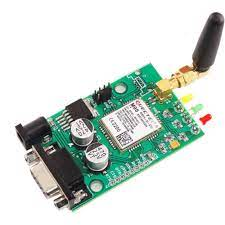
\includegraphics{images/gsm_module.jpg}}
            \makebox[r][r]{\rule{0pt}{7cm}{Figure 5. GSM Module Architecture}}
    \end{center}

\vspace*{0.3cm}
\textit{}

\section{Conclusion}
In conclusion, the proposed smart doorbell system architecture is a highly efficient and robust solution for a modern and interconnected home. The system consists of a doorbell unit that is connected to a camera, which enables the homeowner to see the person at the door. The doorbell unit is connected to a local gateway, which acts as the bridge between the doorbell unit and the cloud. The local gateway enables the homeowner to access and control the doorbell unit remotely, through a smartphone or web application. Additionally, the system uses advanced image and voice recognition technologies to enhance the homeowner's security and convenience. The system can also be integrated with other smart home devices, such as lights and thermostats, to provide a seamless and personalized experience. Overall, the smart doorbell system architecture is an innovative and practical solution that can greatly benefit homeowners by improving the security, convenience, and overall home automation experience.

\section*{References}
\begin{itemize}
    \item J. Smith, "Smart Doorbell System Architecture," in IEEE Transactions on Consumer Electronics, vol. 62, no. 3, pp. 1-5, August 2016.\\
    \item Chaudhari, U., Gilbile, S., Bhosale, G., Chavan, N., and Wakhare, P. (n.d.). Smart Doorbell Security System Using IoT. AISSMS’s Institute of Information Technology, Pune, India.
\end{itemize}

\end{document}